\documentclass[dvipsnames]{beamer}
\usepackage[T1]{fontenc}
\usepackage{geometry}
\usepackage[utf8]{inputenc}
\usepackage{colortbl}
\usepackage[english]{babel}
\usepackage{pgf}
%\usepackage{beamerthemesplit}
\usepackage{graphicx,epsfig, subfigure}
\usepackage{hyperref}
%\usepackage{srcltx}
\usepackage{multirow}
\usepackage{minted}
\definecolor{lightgray}{rgb}{.3,.3,.3}

\usepackage{niceslides}

\title{Proofs as Programs}
\author{Joachim Tilsted Kristensen\\ \texttt{joachim.tilsted@gmail.com}}
\institute{Motorola University}

\date{10/09-2021}

%\setlength{\parskip}{\baselineskip}

\def\Var{\ensuremath{\text{\bf Var}}}
\def\Con{\ensuremath{\text{\bf Con}}}
\def\N{\ensuremath{\mathbb N}}
\def\R{\ensuremath{\mathbb R}}
\def\Q{\ensuremath{\mathbb Q}}
\def\OR{\ensuremath{\ |\ }}
\def\TO{\ensuremath{\rightarrow}}
\def\LB{\ensuremath{\llbracket}}
\def\RB{\ensuremath{\rrbracket}}
\newcommand\LIT[1]{\ensuremath{\text{\tt #1}}}
\newcommand\SLIT[1]{\ \LIT{#1}\ }
\newcommand\IF[3]{\LIT{if}\ #1\ \LIT{then}\ #2\ \LIT{else}\ #3}
\newcommand\INBR[1]{\ensurennmath{\llbracket #1 \rrbracket}}
\def\Eval{\ensuremath \downarrow}

\begin{document}
\frame{\titlepage \vspace{-0.5cm}
}

\begin{frame}
  \frametitle{Curry-Howard isomorphism}

  \begin{block}{Observations:}
    \begin{itemize}
    \item Curry  : Combinator's types are equivalent to axiom-schemes for intuitionistic implicational logic.
    \item Curry  : Hilbert-style deduction systems, coincides with combinatory logic.
    \item Howard : Natural deduction, can be directly interpreted in its intuitionistic version as a typed variant of the lambda calculus.
    \end{itemize}
  \end{block}

  \begin{block}{TLDR:}
    \begin{itemize}
    \item Given a logic, there is a programming language such that every
      given proposition has a corresponding type, and for every proof that a
      proposition holds there is a corresponding program that inhabits the
      type.
    \end{itemize}
  \end{block}

\end{frame}


\frame{
  \frametitle{Lambda Cube ($\lambda_\rightarrow$)}
  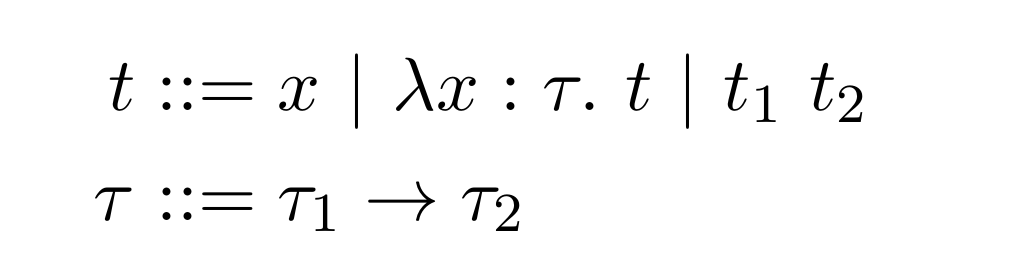
\includegraphics[width=0.5\textwidth]{../figures/illustrations/lambda_calculus/basic_syntax}\\ \\

  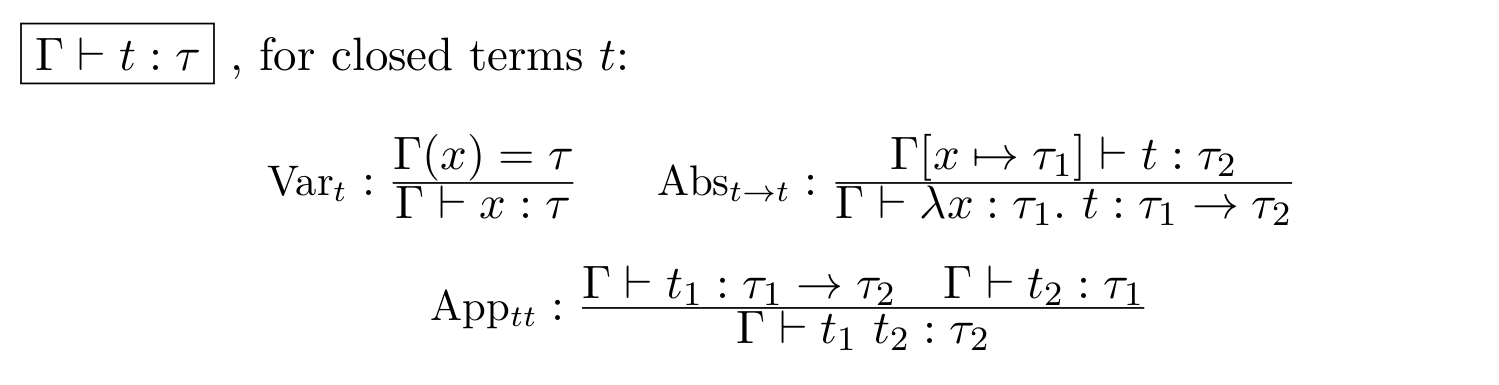
\includegraphics[width=\textwidth]{../figures/illustrations/lambda_calculus/basic_typing}
}

\frame{
  \frametitle{Lambda Cube ($\lambda_2$)}
  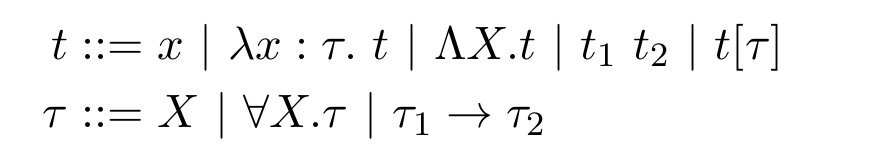
\includegraphics[width=0.5\textwidth]{../figures/illustrations/lambda_calculus/polymorphic_syntax}\\
  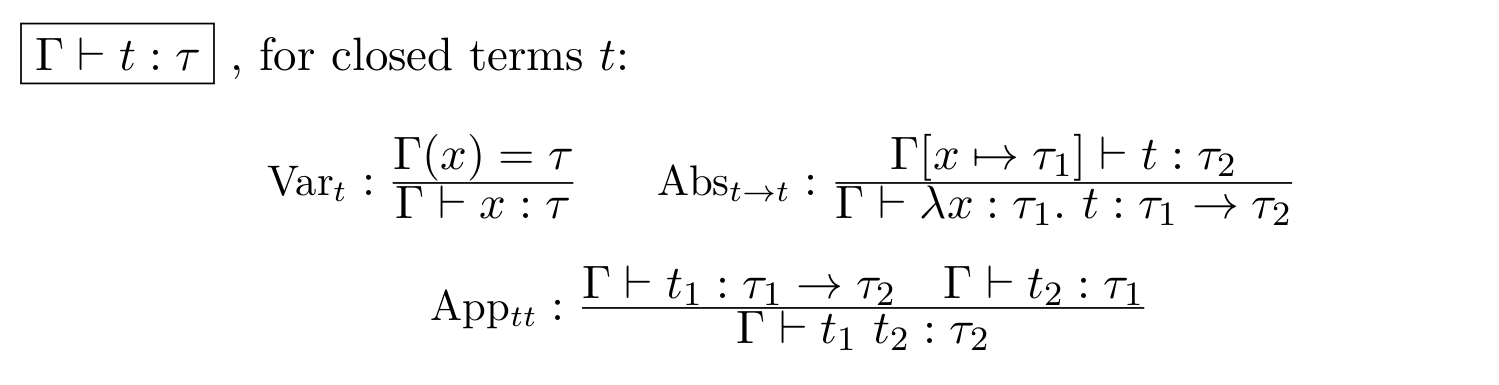
\includegraphics[width=\textwidth]{../figures/illustrations/lambda_calculus/basic_typing}\\
  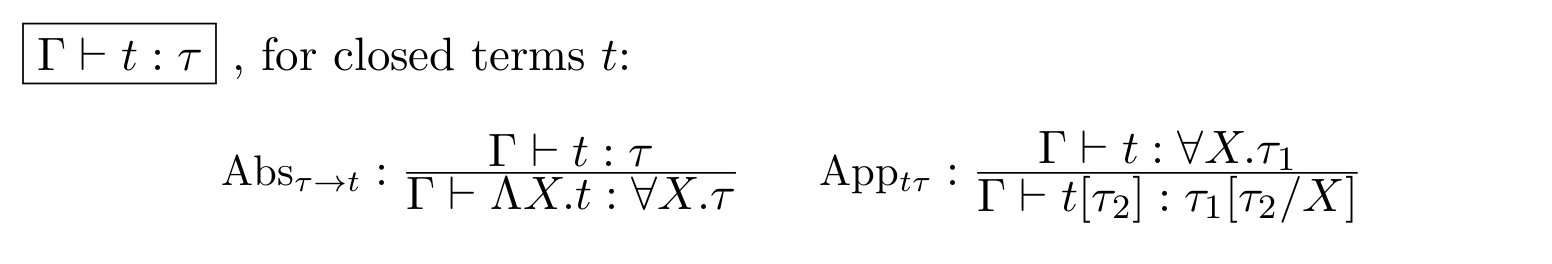
\includegraphics[width=\textwidth]{../figures/illustrations/lambda_calculus/polymorphic_typing}
}

\frame{
  \frametitle{Lambda Cube ($\lambda_\omega$)}
  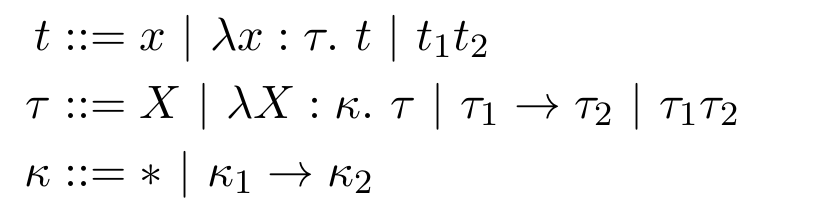
\includegraphics[width=0.5\textwidth]{../figures/illustrations/lambda_calculus/type_level_syntax}\\
  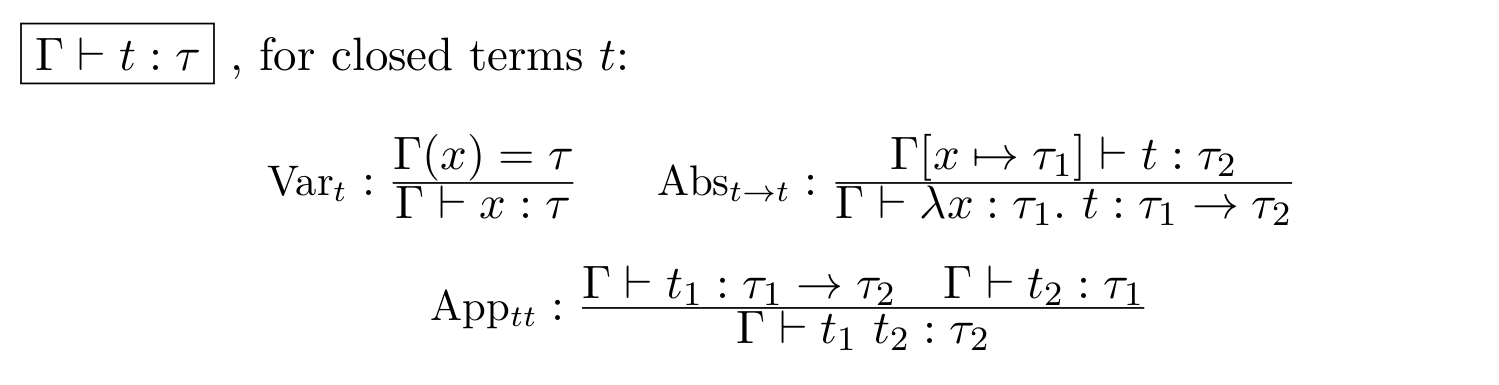
\includegraphics[width=\textwidth]{../figures/illustrations/lambda_calculus/basic_typing}\\

  repeat Var$_t$, Abs$_{t\rightarrow{t}}$ and App$_{tt}$ to get Var$_\tau$, Abs$_{\tau\rightarrow\tau}$ and App$_{\tau\tau}$.
}

\frame{
  \frametitle{Lambda Cube ($\lambda_\Pi$)}
  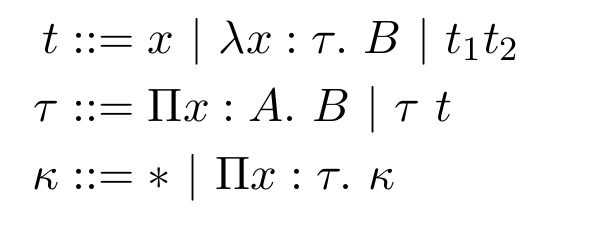
\includegraphics[width=0.5\textwidth]{../figures/illustrations/lambda_calculus/dependent_syntax}\\
  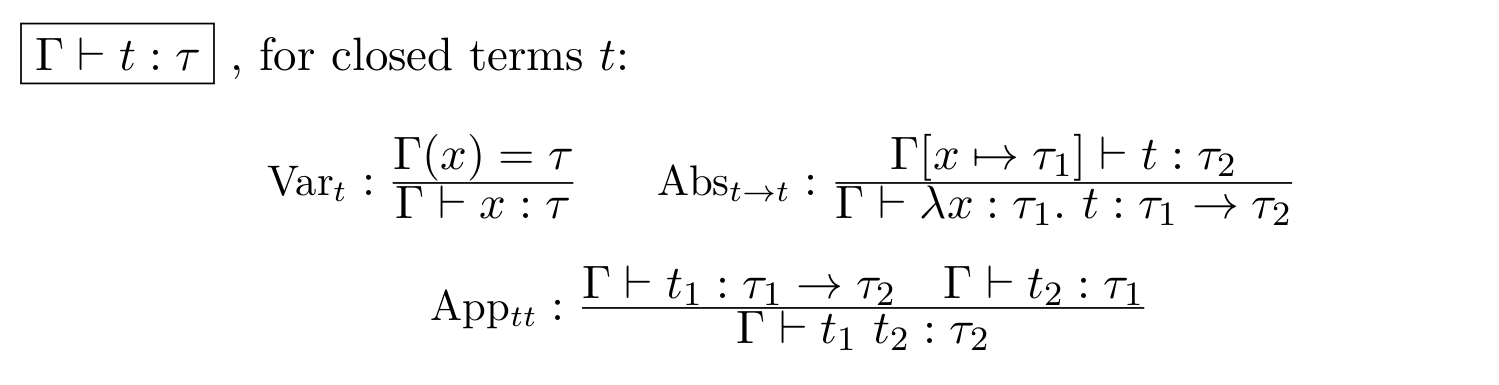
\includegraphics[width=0.9\textwidth]{../figures/illustrations/lambda_calculus/basic_typing}\\
  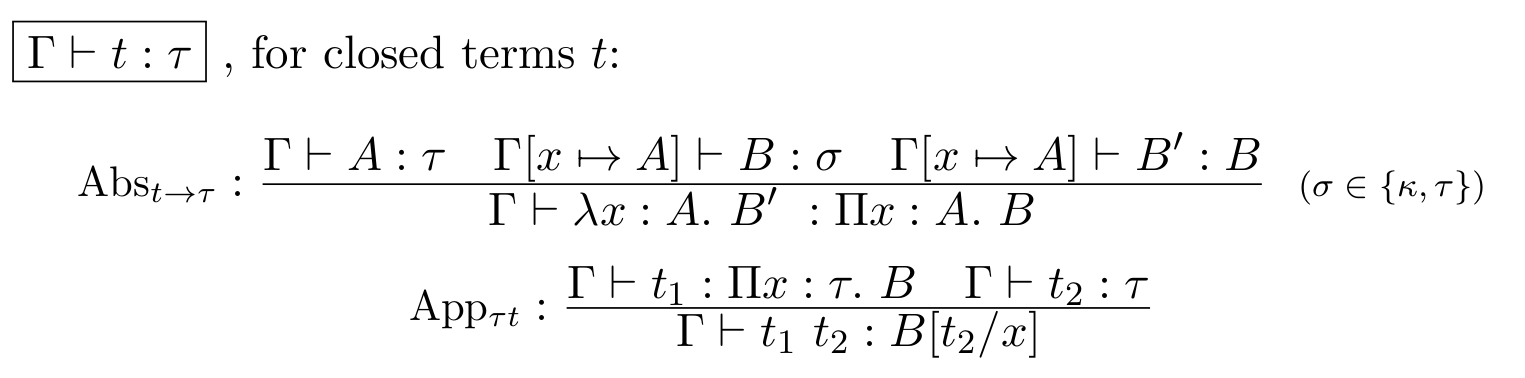
\includegraphics[width=0.9\textwidth]{../figures/illustrations/lambda_calculus/dependent_typing}
}

\begin{frame}
  \Huge\centering
  \intro{Lets write a program. Ehh, I mean proof some stuff.}
\end{frame}

\end{document}

%%% Local Variables:
%%% mode: latex
%%% TeX-master: t
%%% End:
